% http://fachschaft.physik.uni-dortmund.de/images/GlobaltutAP/protokoll.txt
% ========================================
%	Header einbinden
% ========================================

% http://fachschaft.physik.uni-dortmund.de/images/GlobaltutAP/apheader.txt
% ==================================================
%	Festlegung der Dokumentenklasse
% ==================================================


\documentclass[paper=a4, 		% Layout für DinA4
	ngerman				% Deutsche Spracheinstellungen
	]
	{scrartcl} 			% Dokumentklasse für Aufsätze oder z.B. Praktikumsprotokolle

\usepackage{fixltx2e}			% Behebt ein paar Fehler in Latex

% ==================================================
%	Einstellen des Encodings
% ==================================================

\usepackage{ifxetex}
\usepackage{ifluatex} 

\ifxetex
	\usepackage{fontspec}
  	\usepackage{xunicode}
	\usepackage{xltxtra}
    \defaultfontfeatures{Mapping=tex-text} 	% To support LaTeX quoting style
	\setmainfont{Linux Libertine}
=======
    \defaultfontfeatures{Mapping=tex-text} % To support LaTeX quoting style
	\setmainfont{Linux Libertine} % Hier gewünschte Schriftart einfügen
\else
	\ifluatex
		\usepackage{fontspec}		% Falls das nicht funktioniert: \usepackage{luainputenc}
  		\usepackage{xunicode}
  		\defaultfontfeatures{Mapping=tex-text} % To support LaTeX quoting style
		\setmainfont{Linux Libertine} % Hier gewünschte Schriftart einfügen
	\else %pdfTeX
	  \usepackage[utf8]{inputenc}
	  \usepackage[T1]{fontenc}
	 \fi
\fi


% ==================================================
%	Spracheinstellungen
% ==================================================

\usepackage[ngerman]{babel,		% neue deutsche Rechtschreibung
	varioref}			% Bei Referenzen wird der Name des Objektes vor die Refernznummer geschrieben: z.B. \ref{bsp} liefert Seite 1

% ==================================================
%	Referenzen und Links
% ==================================================

\usepackage{hyperref}			% Verlinkungen innerhalb und außerhalb des PDF-Dokuments
\usepackage{url}			% Formattiert URLs, so dass sie sich z.B. besser vom Text abheben
\urlstyle{tt}				% TrueType-Schrift für URLs		



% ==================================================
%	Bibliograhphie
% ==================================================
%Zwei verschiedene Möglichkeiten Bibliographien einzubinden:

%	Möglichkeit 1:
% ========================
	\usepackage[numbers]{natbib}	%Paket für Bibliograhien

	%Bibtex: Nachnamen in Kapitälchen
	%\renewcommand*{\mkbibnamelast}[1]{\textsc{#1}}
	\newcommand*{\mkbibnamelast}[1]{\textsc{#1}}

	% Makros für Anhang + Referenzen
	\newcommand{\anhang}{
		\clearpage		% Anhang auf eine extra Seite packen
		\setcounter{page}{0}	
		\pagenumbering{Roman}	% Anhang wird in römischen Seitenzahlen numeriert
		\appendix		% Kapitelnummerierung in Großbuchstaben statt Zahlen.
	}

	\newcommand{\referenzen}{
		\bibliographystyle{alphadin} 			% Alphabetisch sortiert im DIN-Format
		\addcontentsline{toc}{section}{Referenzen}
		\phantomsection					% Referenzen ins Inhaltsverzeichnis
		\renewcommand{\refname}{\section*{Referenzen}\vspace*{-1em}} % Benennt das Kapitel um
		\bibliography{../include/Bibliographie.bib} 	% Die BibTeX-Datei einbinden
	}
%Zu Verwenden mit \bibliography{BIBDATEI}
% ========================
%	Möglichkeit 2:
% ========================
	%\usepackage{csquotes}				%Wird für Biblatex benötigt
	%\usepackage[style=alphabetic]{biblatex}	%Paket für Bibliograhphien mit Biblatex
%Zu Verwenden mit \bibliography{BIBDATEI} und \printbibliography oder \printbibliography[heading=bibintoc] (falls ein Inhaltsverzeichns verwendet wird)
% ==================================================



% ==================================================
%	Grafiken, Abbildungen und Tabellen
% ==================================================

\usepackage{graphicx}                   % zum Einbinden von Grafiken
\usepackage{xcolor}			% Für die Verwendung von Farben
\usepackage[font=small,			% kleine Schrift für Bildunterschriften
	labelfont=bf			% Fettgedruckte Bildunterschriften
	]
	{caption}			% Für Bildunterschriften

\usepackage{subcaption}			% Für mehrere Objekte nebeneinander mit eigenen Bildunterschriften

\usepackage{tabularx}			% Erweiterte Befehle für Tabellen
\usepackage{booktabs}			% Für professionele Tabellen, siehe Manual
\usepackage{longtable}			% Für Tabellen, die nicht mehr auf eine Seite passen.

\usepackage{rotating}			% Zum Verdrehen von Objekten. Nur mäßig verwenden.

%\graphicspath{{figs/}{bilder/}}	% Bildverzeichnisse MUSS ÜBERPRÜFT WERDEN!!!

% ==================================================
%	Mathematikumgebungen und Einheiten
% ==================================================

\usepackage{amsmath}			% Paket für mathematische Umgebungen und Funktionen
\usepackage{amsfonts}			% Zusätzliche Mathematische Schriftarten
\usepackage{amssymb}			% Zusätzliche Mathematische Symbole
%\usepackage{amscd}			% Zum Setzen Kommutativer Diagramme
\usepackage{amstext}			% Textsatz in der Matheumgebung
\usepackage{upgreek}			% Aufrechte griechische Buchstaben


% Diagramme mit tikz und Gnuplot zeichnen
%	\usepackage{tikz}
%	\usepackage{tikz-qtree}
%	\usepackage{gnuplot-lua-tikz}

% ==================================================
% SIUnitX: Einheiten werden vollautomatisch gesetzt
% ==================================================
\usepackage[
    separate-uncertainty = true, 		% Stellt den Fehler separat dar: Siehe SIUnitX-Manual
    mode 			= text, 	% Stellt Einheiten (Kelvin etc.) Nichtkursiv dar
    quotient-mode	= 	fraction,	% Bruchstriche nutzen
    repeatunits           = false, 
    range-phrase          = {\,bis\,},  
]{siunitx}
\sisetup{
	per-mode = fraction, 			% Bruchstriche nutzen
	output-decimal-marker = {,}, 		% Setzt das Dezimaltrennzeichen als Komma
	multi-part-units = brackets,
	exponent-product = \cdot,
}

\addto\extrasgerman{\sisetup{locale = DE}}	% "Deutsche" Einheiten
\usepackage{cancel}				% Kürzen von Einheiten in SIUnitX ermöglichen


% ==================================================
%	Sonstiges
% ==================================================

%\usepackage[official]{eurosym}			% offizielles Eurosymbol

% ==================================================
%	Seitenlayout
% ==================================================

% Kein Einrücken der Absätze (Einrücken = Null)
	\setlength{\parindent}{0pt}             % kein Einrücken der ersten Zeile in einem neuen Absatz

% Vermeidung von "Schusterjungen"
	\clubpenalty = 3000			% Höchstwert 10000, dann dürfen theoretisch keine Schusterjungen mehr auftreten.
% Vermeidkung von "Hurenkindern"
	\widowpenalty = 3000			% Höchstwert 10000, dann dürfen theoretisch keine Hurenkinder mehr auftreten.
	\displaywidowpenalty = 3000		% Es werden beide Einstellungen benötigt.

% Seitenlayout ändern mit Fancy
	\usepackage{fancyhdr}			% Paket zum bequemeren Verändern des Seitenlayouts

	% Tabellen ändern:
		\renewcommand{\thetable}{\arabic{section}.\arabic{table}} % figures bekommen die richtige Nummerierung: x.y
		\makeatletter \@addtoreset{table}{section} \makeatother      % nach jeder section wird neu gezählt

	% Kapitelüberschriften in der Kopfzeile:
		\renewcommand*{\sectionmark}[1]{\markboth{}{\thesection\ #1}}
		%\renewcommand*{\subsectionmark}[1]{\markboth{}{\thesubsection\ #1}}
		\renewcommand*{\subsectionmark}[1]{\markboth{}{}} % keine Unterüberschriften in der Kopfzeile
		\renewcommand{\plainheadrulewidth}{0.4pt}
	
	% Seitennummern rechts in der Kopfzeile:
		\lhead[\fancyplain{\thepage}{\thepage}]{\fancyplain{}{\rightmark}}
		\rhead[\fancyplain{}{\leftmark}]{\fancyplain{\thepage}{\thepage}}
	
	%Fußzeilen bleiben leer
		\lfoot{}
		\cfoot{}
		\rfoot{}
		
%Eigenes
\usepackage[section]{placeins}
\renewcommand*\rmdefault{iwona}\normalfont\upshape

% ========================================
%	Angaben für das Titelblatt
% ========================================

\title{Versuch\\				% Titel des Versuchs 
\large TU Dortmund, Fakultät Physik\\ 
\normalsize Anfänger-Praktikum}

% \author{Marc Posorske\\			% Name Praktikumspartner A
% {\small \href{marc.posorske@tu-dortmund.de}{marc.posorske@tu-dortmund.de}}	% Erzeugt interaktiven einen Link
% \and						% um einen weiteren Author hinzuzfügen
% Fabian Lehmann\\					% Name Praktikumspartner B
% {\small \href{fabian.lehmann@tu-dortmund.de}{fabian.lehmann@tu-dortmund.de}}		% Erzeugt interaktiven einen Link
% }

\author{Fabian Lehmann\\					% Name Praktikumspartner B
{\small \href{fabian.lehmann@tu-dortmund.de}{fabian.lehmann@tu-dortmund.de}}		% Erzeugt interaktiven einen Link
}

\date{21.Dezember 2012}				% Das Datum der Versuchsdurchführung

% ========================================
%	Das Dokument beginnt
% ========================================

\begin{document}

% ========================================
%	Titelblatt erzeugen
% ========================================

\maketitle					% Jetzt wird die Titelseite erzeugt
\thispagestyle{empty} 				% Weder Kopfzeile noch Fußzeile

% ========================================
%	Der Vorspann
% ========================================

%\newpage					% Wenn Verzeichnisse auf einer neuen Seite beginnen sollen
%\pagestyle{empty}				% Weder Kopf- noch Fußzeile für Verzeichnisse

\tableofcontents

%\newpage					% eine neue Seite
%\thispagestyle{empty}				% Weder Kopf- noch Fußzeile für Verzeichnisse
%\listoffigures					% Abbildungsverzeichnis

%\newpage					% eine neue Seite
%\thispagestyle{empty}				% Weder Kopf- noch Fußzeile für Verzeichnisse
%\listoftables					% Tabellenverzeichnis
\newpage					% eine neue Seite


% ========================================
%	Kapitel
% ========================================

%\section{Einleitung}				% Bei Bedarf
%	Das Geiger-Müller-Zählrohr ist ein Instrument um die Intenstät ionisierender Strahlung zu messen. Seine Funktionsweise basiert darauf, dass wenn $\alpha$-, $\beta$- und $\gamma$-Strahlung in seinem Innern absorbiert wird ein elektrischer Impuls erzeugt wird. Es wird auch heute noch aufgrund seiner einfachen Funktionsweise häufig genutzt.
\FloatBarrier
\section{Theorie}
	Eine wichtige Größe des Magnetismus ist die Suszeptibilität $\chi$, welche die Magnetisierbarkeit 
eines Stoffes in einem Magnetfeld angibt.\\ 
Im Gegensatz zu diamagnetischen Substanzen, deren induzierte magnetische Momente dem Magnetfeld 
entgegengerichtet sind, ist bei paramagnetischen Substanzen die Suszeptibilität positiv.
Diese Eigenschaft hat den Ursprung in einem nicht verschwindenden Drehimpuls, welcher sich aus
den Drehimpulsen der Elektronen, der Elektronenhülle und des Kerns zusammensetzt. Dieser sorgt dafür,
dass sich die magnetischen Momente relativ zum angelegten magnetischen Feld ausrichten. Da diese 
Orientierung durch Bewegung der atomaren Objekte gestört wird, besteht eine Temperaturabhängigkeit
der Suszeptibilität. Im Allgemeinen ist diese nicht trivial von der Temperatur und der magnetischen 
Feldstärke abhängig. Eine konkrete Gleichung für die Berechnung der Suszeptibilität lässt sich
aus der Gleichung für die Magnetisierung unter Zuhilfenahme der Quantenphysik mit Benutzung des 
Landé-Faktors, des Zeeman-Effektes und der Brillouifunktion herleiten. Bei Hochtemperatur lässt
sich $\chi$ passend zum Curieschen Gesetz wie folgt nähern.
\begin{align}
\chi&=\frac{\mu_0 \mu_B^2 g_J^2 N J(J+1)}{3 k T} \\
\chi&=\frac{1}{T}
\end{align}
Starken Paramagnetismus weisen Ionen Seltener Erden auf, diese besitzen innere 4f Elektronen, also 
eine Elektronenhülle mit großen Drehimpulsen. Der Gesamtdrehimpuls $\vec J$ ist dabei durch die
Hundschen Regeln mit dem Pauli-Prinzip \cite{anleitung} festgelegt:
	\begin{table}[h]
	%\begin{description}
			\begin{enumerate}
				\item Gesamtspin $\vec S=\sum \vec s_i$ 
				\item maximaler Drehimpuls $\vec L=\sum \vec l_i$ 
				\item Gesamtdrehimpuls 
				\begin{itemize}
					\item Schale weniger als halbvoll $\vec J=\vec L - \vec S$
					\item Schale mehr als halbvoll $\vec J=\vec L + \vec S$
				\end{itemize}
			\end{enumerate}
	%\end{description}
	\label{hund}
	\end{table}
\FloatBarrier
\section{Durchführung}
	Suszeptibilität lässt sich nicht direkt messen, beeinflusst allerdings die Induktivität einer
Spule nach Gl.\ref{eqspule}.
\begin{align}
&L_m=\mu_0 \frac{n^2 F}{l} + \chi \mu_0 \frac{n^2 Q}{l} \label{eqspule} \\
&F: Spulenquerschnitt, Q: Probenquerschnitt \nonumber
\end{align}
Ein Selektivverstärker filtert Frequenzen, so das Störspannungen zu einem großen Teil ausgeblendet 
werden können. Eine wichtige Eigenschaft dieses Bauteils ist dabei die Güte $Q$, welche beschreibt, 
wann das Verhältnis von $U_A$ zu $U_E$ auf $1/\sqrt{2}$ abgesunken ist.
\begin{align}
Q&=\frac{\nu_0}{\nu_+ - \nu_-} \label{eqn:engute}
\end{align}
	\begin{figure}[h]
		\begin{center}
		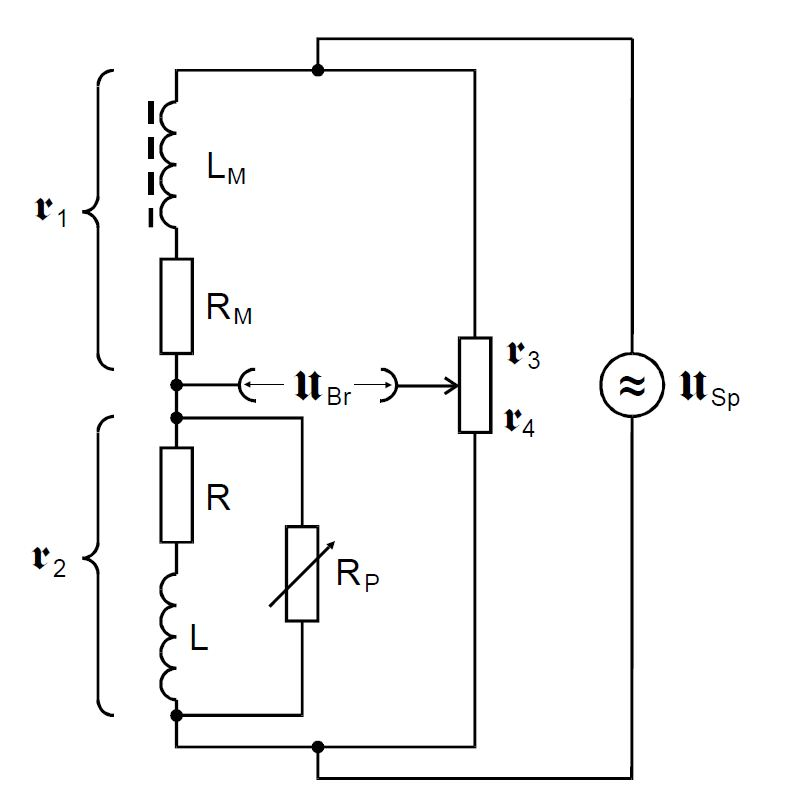
\includegraphics[scale=0.3]{picbrucke.jpg}
		\caption{Brückenschaltung mit Spulen$^{[1]}$}
		\label{picbrucke}
		\end{center}	
	\end{figure}
\FloatBarrier
Um Widerstände zu messen wird häufig eine Brückenschaltung (Abb.\ref{picbrucke}) verwendet. Diese beruht auf dem Prinzip 
Widerstandsverhältnisse zueinander zu messen. Die vier Widerstände, welche in zwei Reihenschaltungen
parallel geschaltet sind werden auf Null abgeglichen bevor der unbekannte Widerstand hinzu kommt. 
Wird als unbekannter Widerstand die bekannte Spule mit Materie gefüllt, so lassen sich folgende Gleichungen
herleiten.
\begin{align}
\chi(U_{Br})&=\frac{U_{Br}}{U_{Sp}}\frac{4l}{\omega \mu_0 n^2 Q} \sqrt{R^2 + \omega^2 (\mu_0 \frac{n^2}{l} F)^2} \\
\text{für } \omega^2 L^2 \gg R^2 : \nonumber \\
\chi(U_{Br})&=4 \frac{F U_{Br}}{Q U_{Sp}} \label{eqchiu}\\ %\label{eqn:chibrucke}\\
\chi(\Delta R)&=2 \frac{\Delta R F}{R_3 Q} \label{eqchir}
\end{align}
%\FloatBarrier
	\begin{figure}[h]
		\begin{center}
		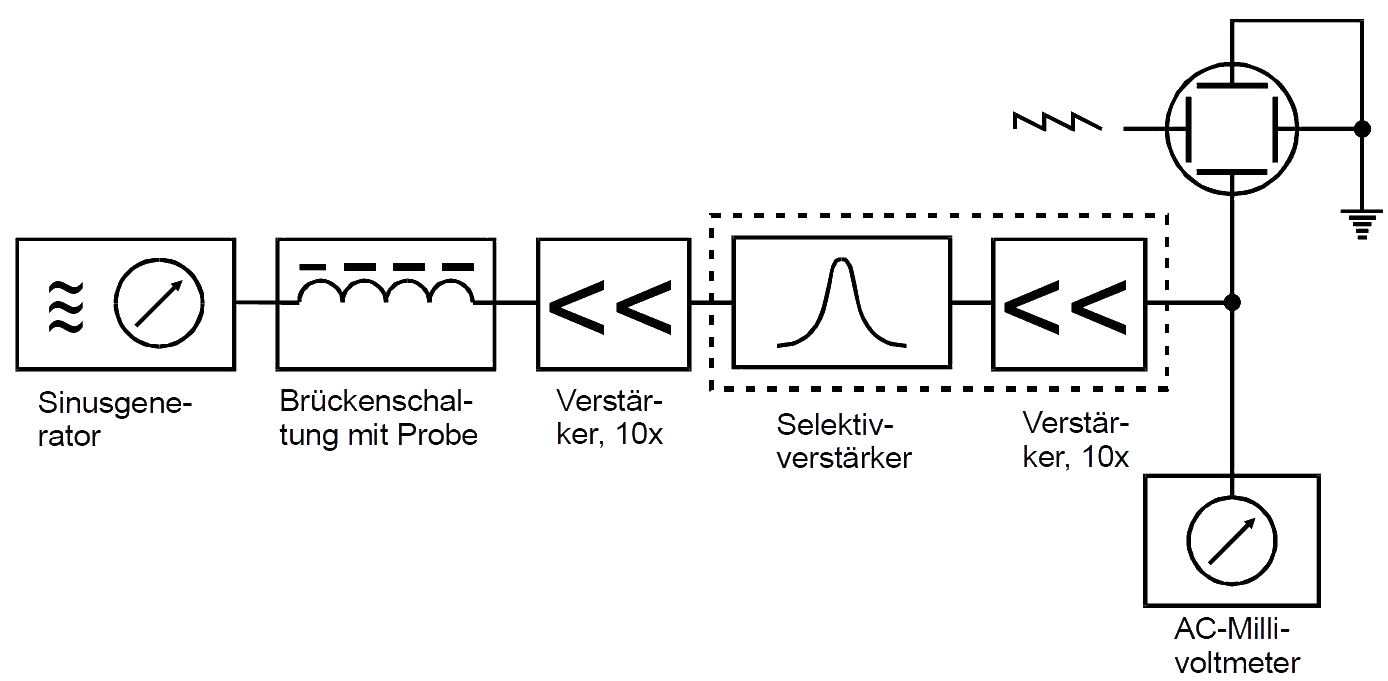
\includegraphics[scale=0.3]{picaufbau.jpg}
		\caption{Aufbau der Messanordnung$^{[1]}$}
		\label{picaufbau}
		\end{center}	
	\end{figure}
Die Messapparatur wurde wie in Abbildung \ref{picaufbau} aufgebaut. Zu Beginn wurde der Selektivverstärker
ausgekoppelt betrachtet um Werte für die Gütekurve aufzuzeichnen. Dabei wurde unter Frequenzvariation bei 
fester Eingangsspannung die Ausgangsspannung abgelesen. \\ 
Um die Verstärkung zu verifizieren wurde dann bei Durchlassfrequenz die selektivverstärkereigene zehnfach 
Verstärkung getestet, sowie die externe zehnfach Verstärkung überprüft.\\
Darauf folgend wurden die Elemente wieder eingekoppelt (Abb.\ref{picaufbau}) und es wurde mit einem anderen 
Sinusgenerator die Proben von $Nd_2O_3$,$Gd_2O_3$ und $Dy_2O_3$ untersucht. Dabei wurde die Brückenschaltung
jeweils zuerst auf Null abgeglichen, dann die Probe eingeführt und abermals auf Null abgeglichen.


\section{Auswertung}
	\subsection{Kennlinien der Hochvakuumdiode} 
Aus den Tabellen (\ref{taba1} - \ref{taba5}) sind die darauf folgenden 
Abbildungen (\ref{pica1} - \ref{pica5}) erstellt worden.
\begin{table}[h!]
	\begin{center}
		\begin{tabular}{cc}
			Anodenspannung [V] & Anodenstrom [mA]\\ \hline
			10	&0,044\\
			20	&0,088\\
			30	&0,108\\
			40	&0,119\\
			50	&0,126\\
			60	&0,128\\
			70	&0,132\\
			80	&0,135\\
			90	&0,138\\
			100	&0,141\\
			110	&0,144\\
			120	&0,146\\
			130	&0,147\\
			140	&0,149\\
			150	&0,150\\
			160	&0,151\\
			170	&0,152\\
			180	&0,154\\
			190	&0,155\\
			200	&0,156\\
			210	&0,157
		\end{tabular}
		\caption{Kennlinie 1 (Heizwerte: 4,2V; 2,1A)}
		\label{taba1}
	\end{center}
\end{table} \begin{table}[h]
	\begin{center}
		\begin{tabular}{cc}
			Anodenspannung [V] & Anodenstrom [mA]\\ \hline
			10	&0,049\\
			20	&0,123\\
			30	&0,181\\
			40	&0,232\\
			50	&0,263\\
			60	&0,281\\
			70	&0,302\\
			80	&0,310\\
			90	&0,322\\
			100	&0,330\\
			110	&0,336\\
			120	&0,340\\
			130	&0,344\\
			140	&0,348\\
			150	&0,352\\
			160	&0,355\\
			170	&0,359\\
			180	&0,362\\
			190	&0,366\\
			200	&0,368\\
			210	&0,371\\
			220	&0,373\\
			230	&0,375\\
			240	&0,377\\
			250	&0,380
		\end{tabular}
		\caption{Kennlinie 2 (Heizwerte: 4,8V; 2,2A)}
		\label{taba2}
	\end{center}
\end{table} \begin{table}[h]
	\begin{center}
		\begin{tabular}{cc}
			Anodenspannung [V] & Anodenstrom [mA]\\ \hline
			10	&0,050\\
			20	&0,135\\
			30	&0,230\\
			40	&0,309\\
			50	&0,367\\
			60	&0,421\\
			70	&0,479\\
			80	&0,525\\
			90	&0,555\\
			100	&0,589\\
			110	&0,622\\
			120	&0,642\\
			130	&0,655\\
			140	&0,665\\
			150	&0,671\\
			160	&0,677\\
			170	&0,682\\
			180	&0,686\\
			190	&0,692\\
			200	&0,697\\
			210	&0,702\\
			220	&0,706\\
			230	&0,709\\
			240	&0,713\\
			250	&0,717
		\end{tabular}
		\caption{Kennlinie 3 (Heizwerte: 5,0V; 2,3A)}
		\label{taba3}
	\end{center}
\end{table} \begin{table}[h]
	\begin{center}
		\begin{tabular}{cc}
			Anodenspannung [V] & Anodenstrom [mA]\\ \hline
			10	&0,061\\
			20	&0,163\\
			30	&0,275\\
			40	&0,383\\
			50	&0,460\\
			60	&0,575\\
			70	&0,689\\
			80	&0,812\\
			90	&0,947\\
			100	&1,042\\
			110	&1,131\\
			120	&1,229\\
			130	&1,343\\
			140	&1,452\\
			150	&1,566\\
			160	&1,666\\
			170	&1,779\\
			180	&1,882\\
			190	&1,984\\
			200	&2,08\\
			210	&2,18\\
			220	&2,28\\
			230	&2,37\\
			240	&2,45\\
			250	&2,53
		\end{tabular}
		\caption{Kennlinie 4 (Heizwerte: 5,9V; 2,5A)}
		\label{taba4}
	\end{center}
\end{table} \begin{table}[h]
	\begin{center}
		\begin{tabular}{cc}
			Anodenspannung [V] & Anodenstrom [mA]\\ \hline
			10	&0,063\\
			20	&0,170\\
			30	&0,288\\
			40	&0,398\\
			50	&0,514\\
			60	&0,606\\
			70	&0,711\\
			80	&0,829\\
			90	&0,958\\
			100	&1,107\\
			110	&1,282\\
			120	&1,399\\
			130	&1,494\\
			140	&1,593\\
			150	&1,730\\
			160	&1,865\\
			170	&2,00\\
			180	&2,14\\
			190	&2,29\\
			200	&2,44\\
			210	&2,58\\
			220	&2,72\\
			230	&2,86\\
			240	&3,00\\
			250	&3,11
		\end{tabular}
		\caption{Kennlinie 5 (Heizwerte: 6,1V; 2,6A)}
		\label{taba5}
	\end{center}
\end{table}
	\begin{figure}[h]
		\begin{center}
		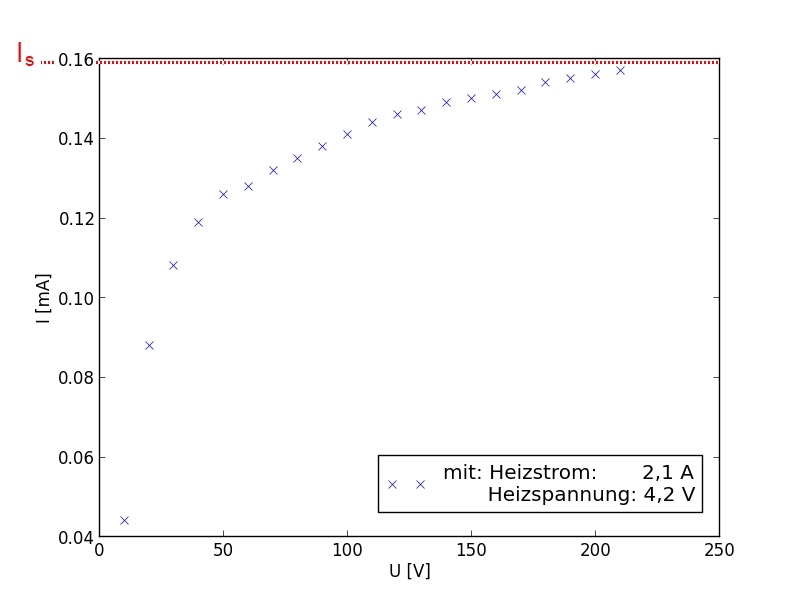
\includegraphics[scale=0.75]{pica1.jpg}
		\caption{Kennlinie 1 (Heizwerte: 4,2V; 2,1A)}
		\label{pica1}
		\end{center}	
	\end{figure} 	\begin{figure}[h]
		\begin{center}
		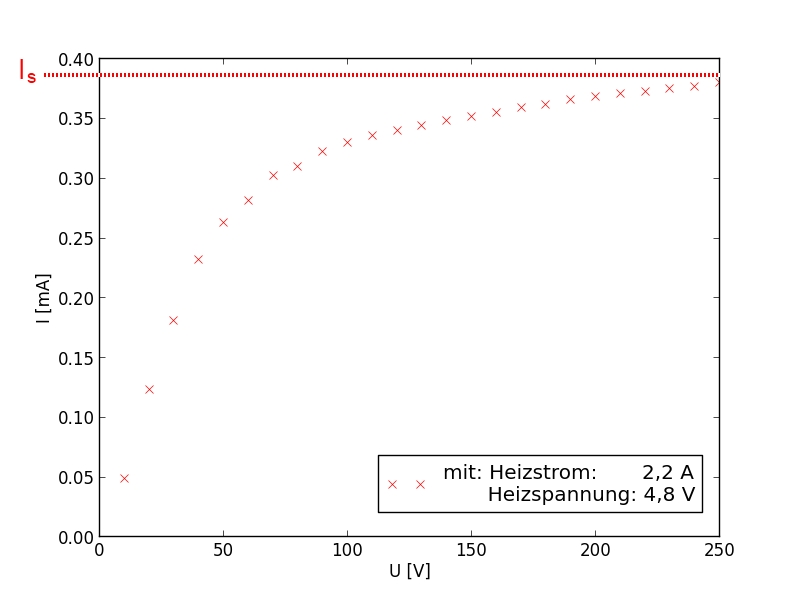
\includegraphics[scale=0.75]{pica2.jpg}
		\caption{Kennlinie 2 (Heizwerte: 4,8V; 2,2A)}
		\label{pica2}
		\end{center}	
	\end{figure} 	\begin{figure}[h]
		\begin{center}
		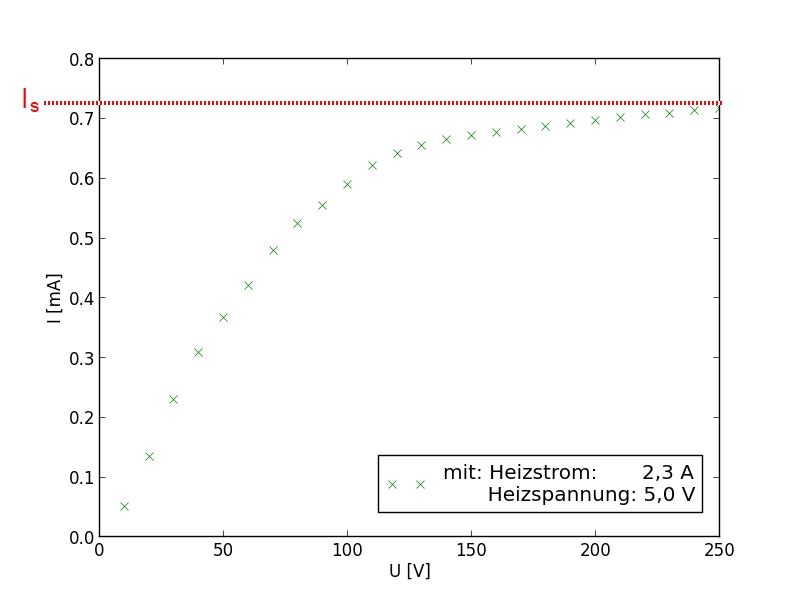
\includegraphics[scale=0.75]{pica3.jpg}
		\caption{Kennlinie 3 (Heizwerte: 5,0V; 2,3A)}
		\label{pica3}
		\end{center}	
	\end{figure} 	\begin{figure}[h]
		\begin{center}
		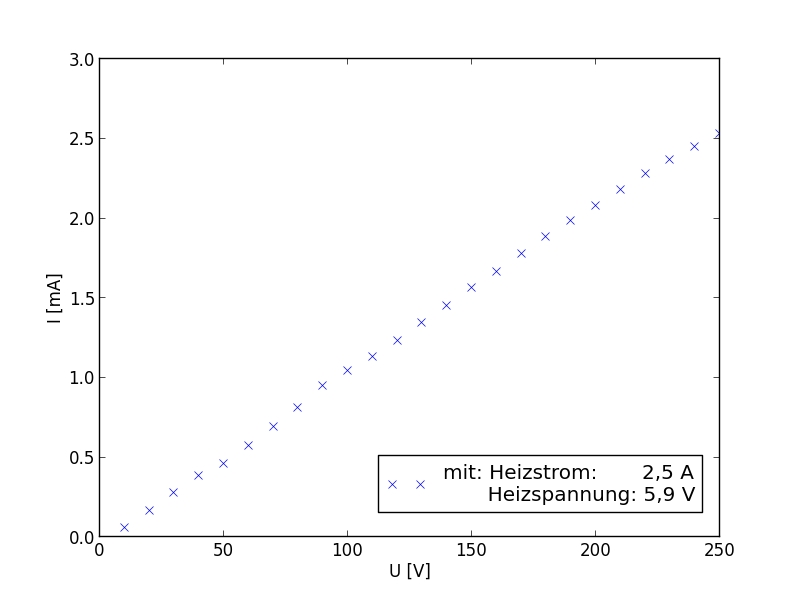
\includegraphics[scale=0.75]{pica4.jpg}
		\caption{Kennlinie 4 (Heizwerte: 5,9V; 2,5A)}
		\label{pica4}
		\end{center}	
	\end{figure} 	\begin{figure}[h]
		\begin{center}
		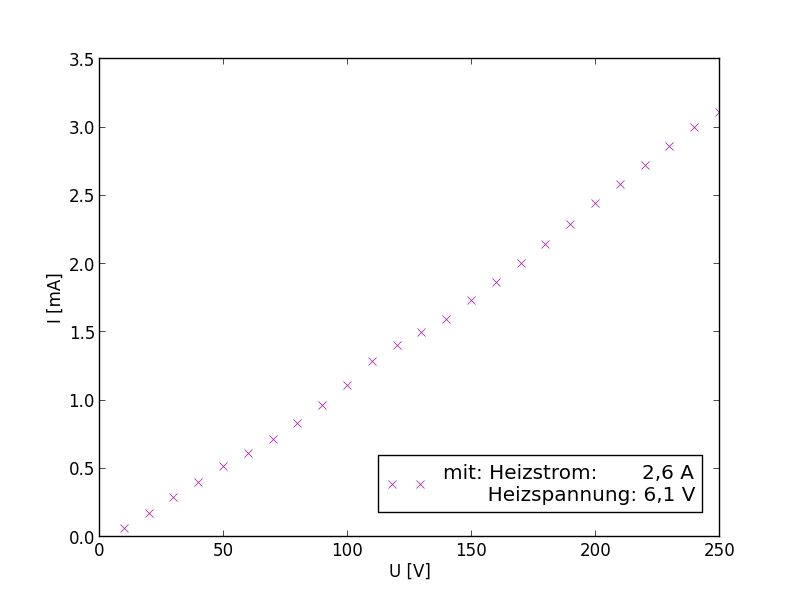
\includegraphics[scale=0.75]{pica5.jpg}
		\caption{Kennlinie 5 (Heizwerte: 6,1V; 2,6A)}
		\label{pica5}
		\end{center}	
	\end{figure} 
Aus den Abbildungen \ref{pica1},\ref{pica2} und \ref{pica3} wurde der Sättingungsstrom 
$I_s$ abgelesen (Tab. \ref{tabis}). Bei den Abbildungen \ref{pica4} und \ref{pica5} war das 
nicht möglich, der Großteil des Sättigungsstromgebietes befand sich außerhalb der 
Messwerte.
\begin{table}[h]
	\begin{center}
		\begin{tabular}{ccc}
			Heizspannung [V] & Heizstrom [A] & Sättigungsstrom [mA]\\ \hline
			4,2 &2,1 &0,16\\
			4,8 &2,2 &0,38\\
			5,0 &2,3 &0,72
		\end{tabular}
		\caption{Sättigungstromwerte}
		\label{tabis}
	\end{center}
\end{table}
\FloatBarrier
\subsection{Langmuir-Schottkysches-Gesetz}
Das Langmuir-Schottkysche Raumladungsgesetz (Gl. \ref{eqlangmuir}) ist solange gültig, bis sich die Kennlinie
dem Sättigungstrom annähert, also das Raumladungsgebiet in das Sättigungsstromgebiet 
übergeht. Für die maximal mögliche Heizleistung passiert das ungefähr bei 200V.
Trägt man die Messwerte logarithmisch auf, so lässt sich der Exponent erkennen (vgl. 
Abb. \ref{picb1}). Der Exponent berechnet sich durch lineare Regression \cite{linreg}
aus Gleichung \ref{eqb1}, beziehungsweise Tabelle \ref{tabblinreg}, welche auf Tabelle \ref{taba5} aufbaut.
\begin{align}
I&\sim U^\alpha \\
\Rightarrow ln(I)&\sim ln(U)*\alpha \label{eqb1}
\end{align}
\begin{table}[h]
	\begin{center}
		\begin{tabular}{cccc}
			U[V] & I[mA] & ln(U) & ln(I)\\ \hline
			10	&0,063& 2,30& -2,765\\                  
			20	&0,170& 2,99& -1,772\\
			30	&0,288& 3,40& -1,245\\
			40	&0,398& 3,68& -0,921\\
			50	&0,514& 3,91& -0,666\\
			60	&0,606& 4,09& -0,501\\
			70	&0,711& 4,24& -0,341\\
			80	&0,829& 4,38& -0,188\\
			90	&0,958& 4,49& -0,043\\
			100	&1,107& 4,60& 0,102\\
			110	&1,282& 4,70& 0,248\\
			120	&1,399& 4,78& 0,336\\
			130	&1,494& 4,86& 0,402\\
			140	&1,593& 4,94& 0,466\\
			150	&1,730& 5,01& 0,548\\
			160	&1,865& 5,07& 0,623\\
			170	&2,000& 5,13& 0,693\\
			180	&2,140& 5,19& 0,761\\
			190	&2,290& 5,24& 0,829\\
		\end{tabular}
		\caption{Logarithmen zur Kennlinie 5 (Heizwerte: 6,1V; 2,6A)}
		\label{tabblinreg}
	\end{center}
\end{table}
\FloatBarrier
Aus der linearen Regression nach \cite{linreg} berechnet sich der gesuchte Exponent $\alpha$ beziehungsweise die Ausgleichskurve (Abb. \ref{picb1}).
\begin{align}
t&=a*x+b \\
a&=\alpha=1,18 \\
b&=-5.3443 \\
\Rightarrow I&=U^\alpha*e^b 
\end{align}
	\begin{figure}[h]
		\begin{center}
		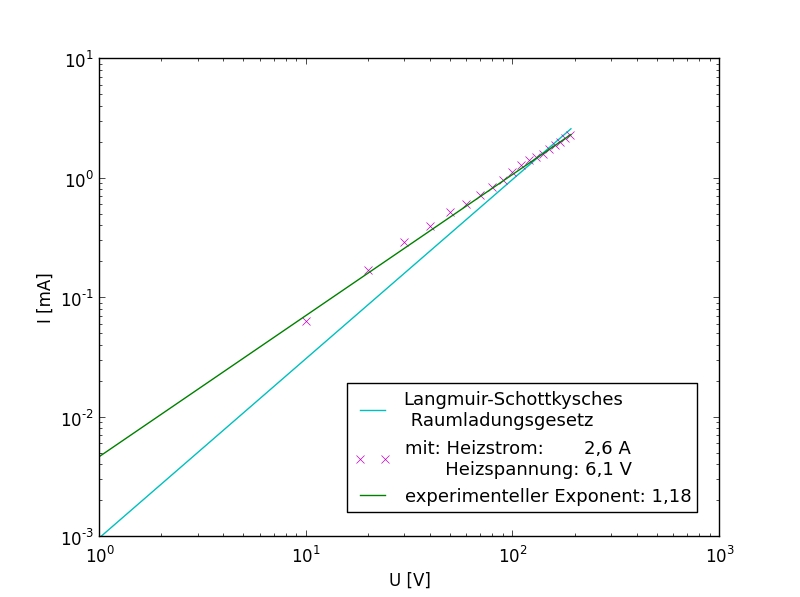
\includegraphics[scale=0.75]{picb1.jpg}
		\caption{Strom-Spannungs-Beziehung}
		\label{picb1}
		\end{center}	
	\end{figure}
\FloatBarrier
\subsection{Kathodentemperatur im Anlaufstromgebiet}
Aus den aufgezeichneten Messwerten (vgl. Tab. \ref{tabc1}) lässt sich nach der Gleichung \ref{eqcureal}
die angezeigte Spannung $U_{Heiz}$ nach $U_{Heiz,real}$ korrigieren. Daraus lässt sich dann mit 
Gleichung \ref{eqtemp} T berechnen (Tab. \ref{tabc1}). Die genutzen Apparaturkonstanten waren dabei:
\begin{align}
\begin{split}
f&=0,335cm^2 \label{eqdatatemp}\\
\eta&=0,28\\
N_{WL}&=0,95W .
\end{split}
\end{align} 
Die Werte sind in Abbildung \ref{picc1} veranschaulicht.
\begin{align}
U_{Heiz,real}&=U_{Heiz}-R*I_S \label{eqcureal}\\
mit: R&=1M\Omega \\
\end{align}
\begin{table}[h]
	\begin{center}
		\begin{tabular}{cc}
			$6{,}1V-U_{Heiz,real}$[$\mu$V]&2298K-T[$\mu$K] \\ \hline
			0,11&207 \\
			0,091&205\\
			0,065&202\\
			0,045&200\\
			0,030&199\\
			0,020&198\\
			0,013&197\\
			0,0075&197\\
			0,0045&196\\
			0,0029&196\\
			0,0017&196
		\end{tabular}
		\caption{Kathodentemperatur im Anlaufstromgebiet($U_{Heiz}=6,1V$)}
		\label{tabc1}
	\end{center}
\end{table} 	\begin{figure}[h]
		\begin{center}
		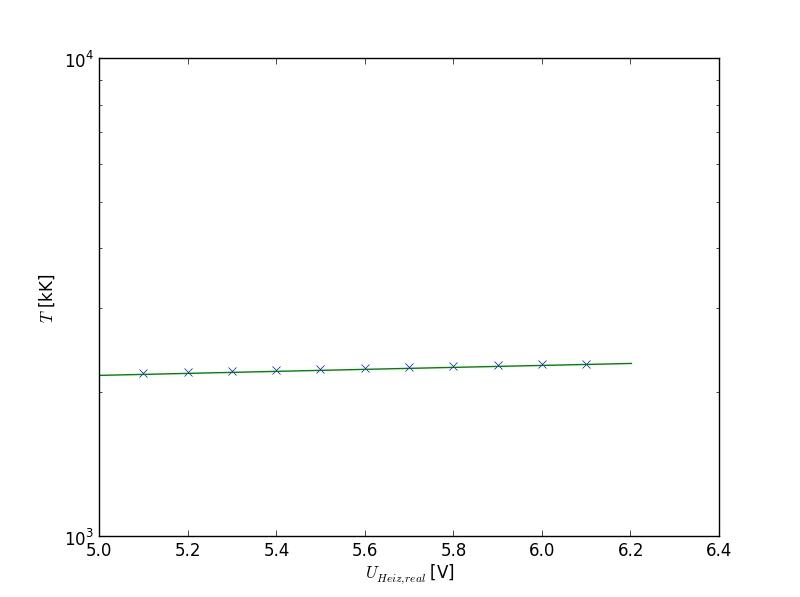
\includegraphics[scale=0.75]{picc1.jpg}
		\caption{Kathodentemperatur im Anlaufstromgebiet}
		\label{picc1}
		\end{center}	
	\end{figure}
\FloatBarrier
\subsection{Kathodentemperatur bei Saugspannung}
Die Leistungbilanz des Heizstromkreises dient nach Gleichung \ref{eqtemp} mit den Werten aus \ref{eqdatatemp}
zur Berechnung der Temperatur aus den aufgezeichneten Werten (vgl. Tab. \ref{taba1}-\ref{taba5}). Die Ergebnisse
sind in Tabelle \ref{tabd1} und in Abbildung \ref{picd1} dargestellt. 
\begin{table}[h]
	\begin{center}
		\begin{tabular}{cc}
			U[V]&$\Delta Q [\frac{\text{C}}{e}] * 10^9$ \\ \hline
			339&63,68\\
			342&11,50\\
			345&13,53\\
			348&12,40\\
			351&13,25\\
			354&12,39\\
			357&11,92\\
			360&12,01\\
			410&18,17\\
			460&24,10\\
			510&30,09\\
			560&35,97\\
			610&41,55\\
			650&47,73\\
			653&48,29\\
			656&46,66\\
			659&48,33\\
			662&46,36\\
			665&52,44\\
			668&52,20\\
			671&52,79\\
			674&53,75\\
			677&50,56\\
			680&51,58\\
			683&50,60\\
			686&54,91\\
			689&49,79\\
			692&48,88\\
			695&50,28\\
			698&46,15\\
			701&52,62
		\end{tabular}
		\caption{freigesetzte Ladungsmenge im Zählrohr}
		\label{tabd1}
	\end{center}
\end{table} 	\begin{figure}[h]
		\begin{center}
		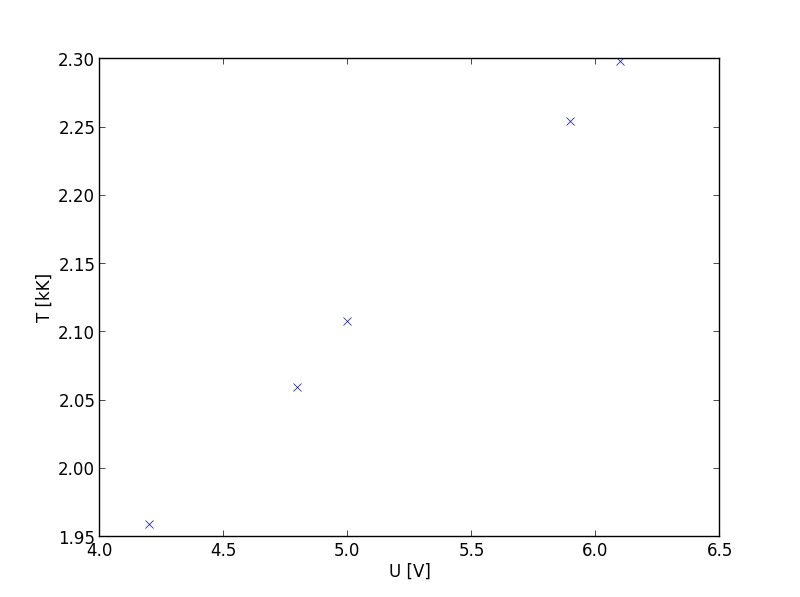
\includegraphics[scale=0.75]{picd1.jpg}
		\caption{Kathodentemperatur unter Heizleistungsvariation}
		\label{picd1}
		\end{center}	
	\end{figure}
\FloatBarrier
\subsection{Austrittsarbeit des Kathodenmaterials}
Um die Austrittsarbeit der Wolfram-Kathode nach der Richardson-Gleichung \ref{eqrichard} zu berechnen,
werden die T Werte aus Tabelle \ref{tabd1} und die Sättigungsstromwerte aus Tabelle \ref{tabis}
verwendet. Die Ergebnisse für die Austrittsarbeit $e_o\varphi$ sind in Tabelle \ref{tabe1} zusammengefasst.
Der Mittelwert der Austrittsarbeit $\overline{e_o\varphi}$, welcher nach Gleichung \ref{eqmittwert} berechnet
wird, beträgt:
\begin{align}
\overline{e_o\varphi}&=6{,}5\overline{3}\\
\overline{x}&=\frac{1}{N}\sum\limits_{i=1}^N x_i \label{eqmittwert}
\end{align}
\begin{table}[h]
	\begin{center}
		\begin{tabular}{cc}
			$I_S$[mA]& $e_0\varphi$[eV] \\ \hline
			0,16&4,71\\
			0,38&4,81\\
			0,72&4,82\\
			2,80&4,91\\
			3,50&4,97
		\end{tabular}
		\caption{Austrittsarbeit (Wolfram)}
		\label{tabe1}
	\end{center}
\end{table}
\FloatBarrier


\section{Diskussion}
	\subsection{Innenwiderstand und Leerlaufspannung}
Waren die verschiedenen Probleme durch defekte Versuchsgeräte ausgeräumt, so waren die einzelnen
Messungen immer noch recht ungenau, da teilweise neben den Ablesefehlern auch noch ein Knopf zur Aktivierung des
Belastungswiderstands gedrückt werden musste, dabei hing der Belastungswiderstand von der Kraft des Druckes ab.
\begin{align}
U_{0,direkt}&=1,575 \text{ V} \\
\Delta U_{0,direkt}&=1,0368*10^{-6}\text{ V}\\
U_{0,belastet}&=(1.5927\pm 0.0205)\text{ V}\\
R_{i,belastet}&=(6.5829\pm 0.1742)\Omega\\
U_{0,belastet + gegen}&=(1.6662\pm 0.0320)\text{ V}\\
R_{i,belastet + gegen}&=(6.6078\pm 0.2212)\Omega
\end{align}
Der Wert der direkten Messung der Leerlaufspannung der Monozelle 
passt gut zu den errechneten Werten der linearen Regression der Monozelle. Dabei ist anzumerken, dass die direkte Messung
im Gegensatz zu den anderen Messreihen nur auf einem einzelnen Wert beruht. Der aus den Messreihen erkennbare Unterschied des Innenwiderstands liegt nicht einmal im einstelligen Prozentbereich, woraus sich auf eine einigermaßen gute Genauigkeit schließen lässt.\\
Bei den zwei anderen Spannungsquellen lassen sich folgende Ergebnisse festhalten:
\begin{align}
R_{i,Rechteckspannung}&=(48.1232\pm 1.1149)\Omega\\
U_{0,Rechteckspannung}&=(0.5728\pm 0.0050)\text{ V}\\
R_{i,Sinusspannung}&=(535.9086\pm 4.5713)\Omega\\
U_{0,Sinusspannung}&=(1.8024\pm 0.0069)\text{ V}
\end{align}
Bei dem Vergleich mit den Werten der Monozelle zeigt sich, dass bei deutlich größerem Innenwiderstand der
Rechtecksspannungsquelle die Leerlaufspannung wesentlich kleiner ist. Die Leerlaufspannung der
Sinusspannungsquelle ist größer als diee der Monozelle, jedoch ist der Innenwiderstand noch viel
größer als der Innenwiderstand der Rechtecksspannungsquelle. Diese Ergebnisse weisen auf einen 
komplexeren Zusammenhang zwischen den einzelnen Größen.
\subsection{Der systematische Fehler}
Wird das Voltmeter hinter dem Amperemeter angelegt, also sozusagen um das Amperemeter
herum, so wird natürlich nur die durch das Amperemeter verursachte Spannung gemessen, welche je
nach Güte des Amperemeters verschieden kleine Werte besitzt, jedoch nicht die eigentlich
zu messende Spannung $U_k$ widerspiegelt.\\
Wird das Voltmeter hinter dem Amperemeter angelegt, also sozusagen um den Belastungswiderstand,
so misst das Amperemeter nicht nur den Strom, der durch den Belastungswiderstand fließt, sondern
auch den je nach Güte des Voltmeters verschieden kleinen Strom, welcher durch das Voltmeter selbst
fließt. Das führt ebenfalls zu einem verfälschten Messergebnis.
\subsection{Die umgesetzte Leistung im Belastungswiderstand}
Aus Abbildung \ref{pice} wird deutlich, dass die Messwerte relativ gut zu den aus der Theorie erwarteten
Werten passen. Bis auf ein paar vermutliche Mesungenauigkeiten kann nicht ohne weiteres auf eine 
systematische Abweichung geschlossen werden. Gut erkennbar ist auch das Maximum der Kurve. Die maximale Leistung scheint bei einem Widerstand von $R_{a,max}=7\Omega$ erreicht zu werden.
% ========================================
%	Literaturverzeichnis
% ========================================

\bibliographystyle{plainnat}			% Bibliographie-Style auswählen
\bibliography{lib}			% Literaturverzeichnis

% ========================================
%	Das Dokument endent
% ========================================
%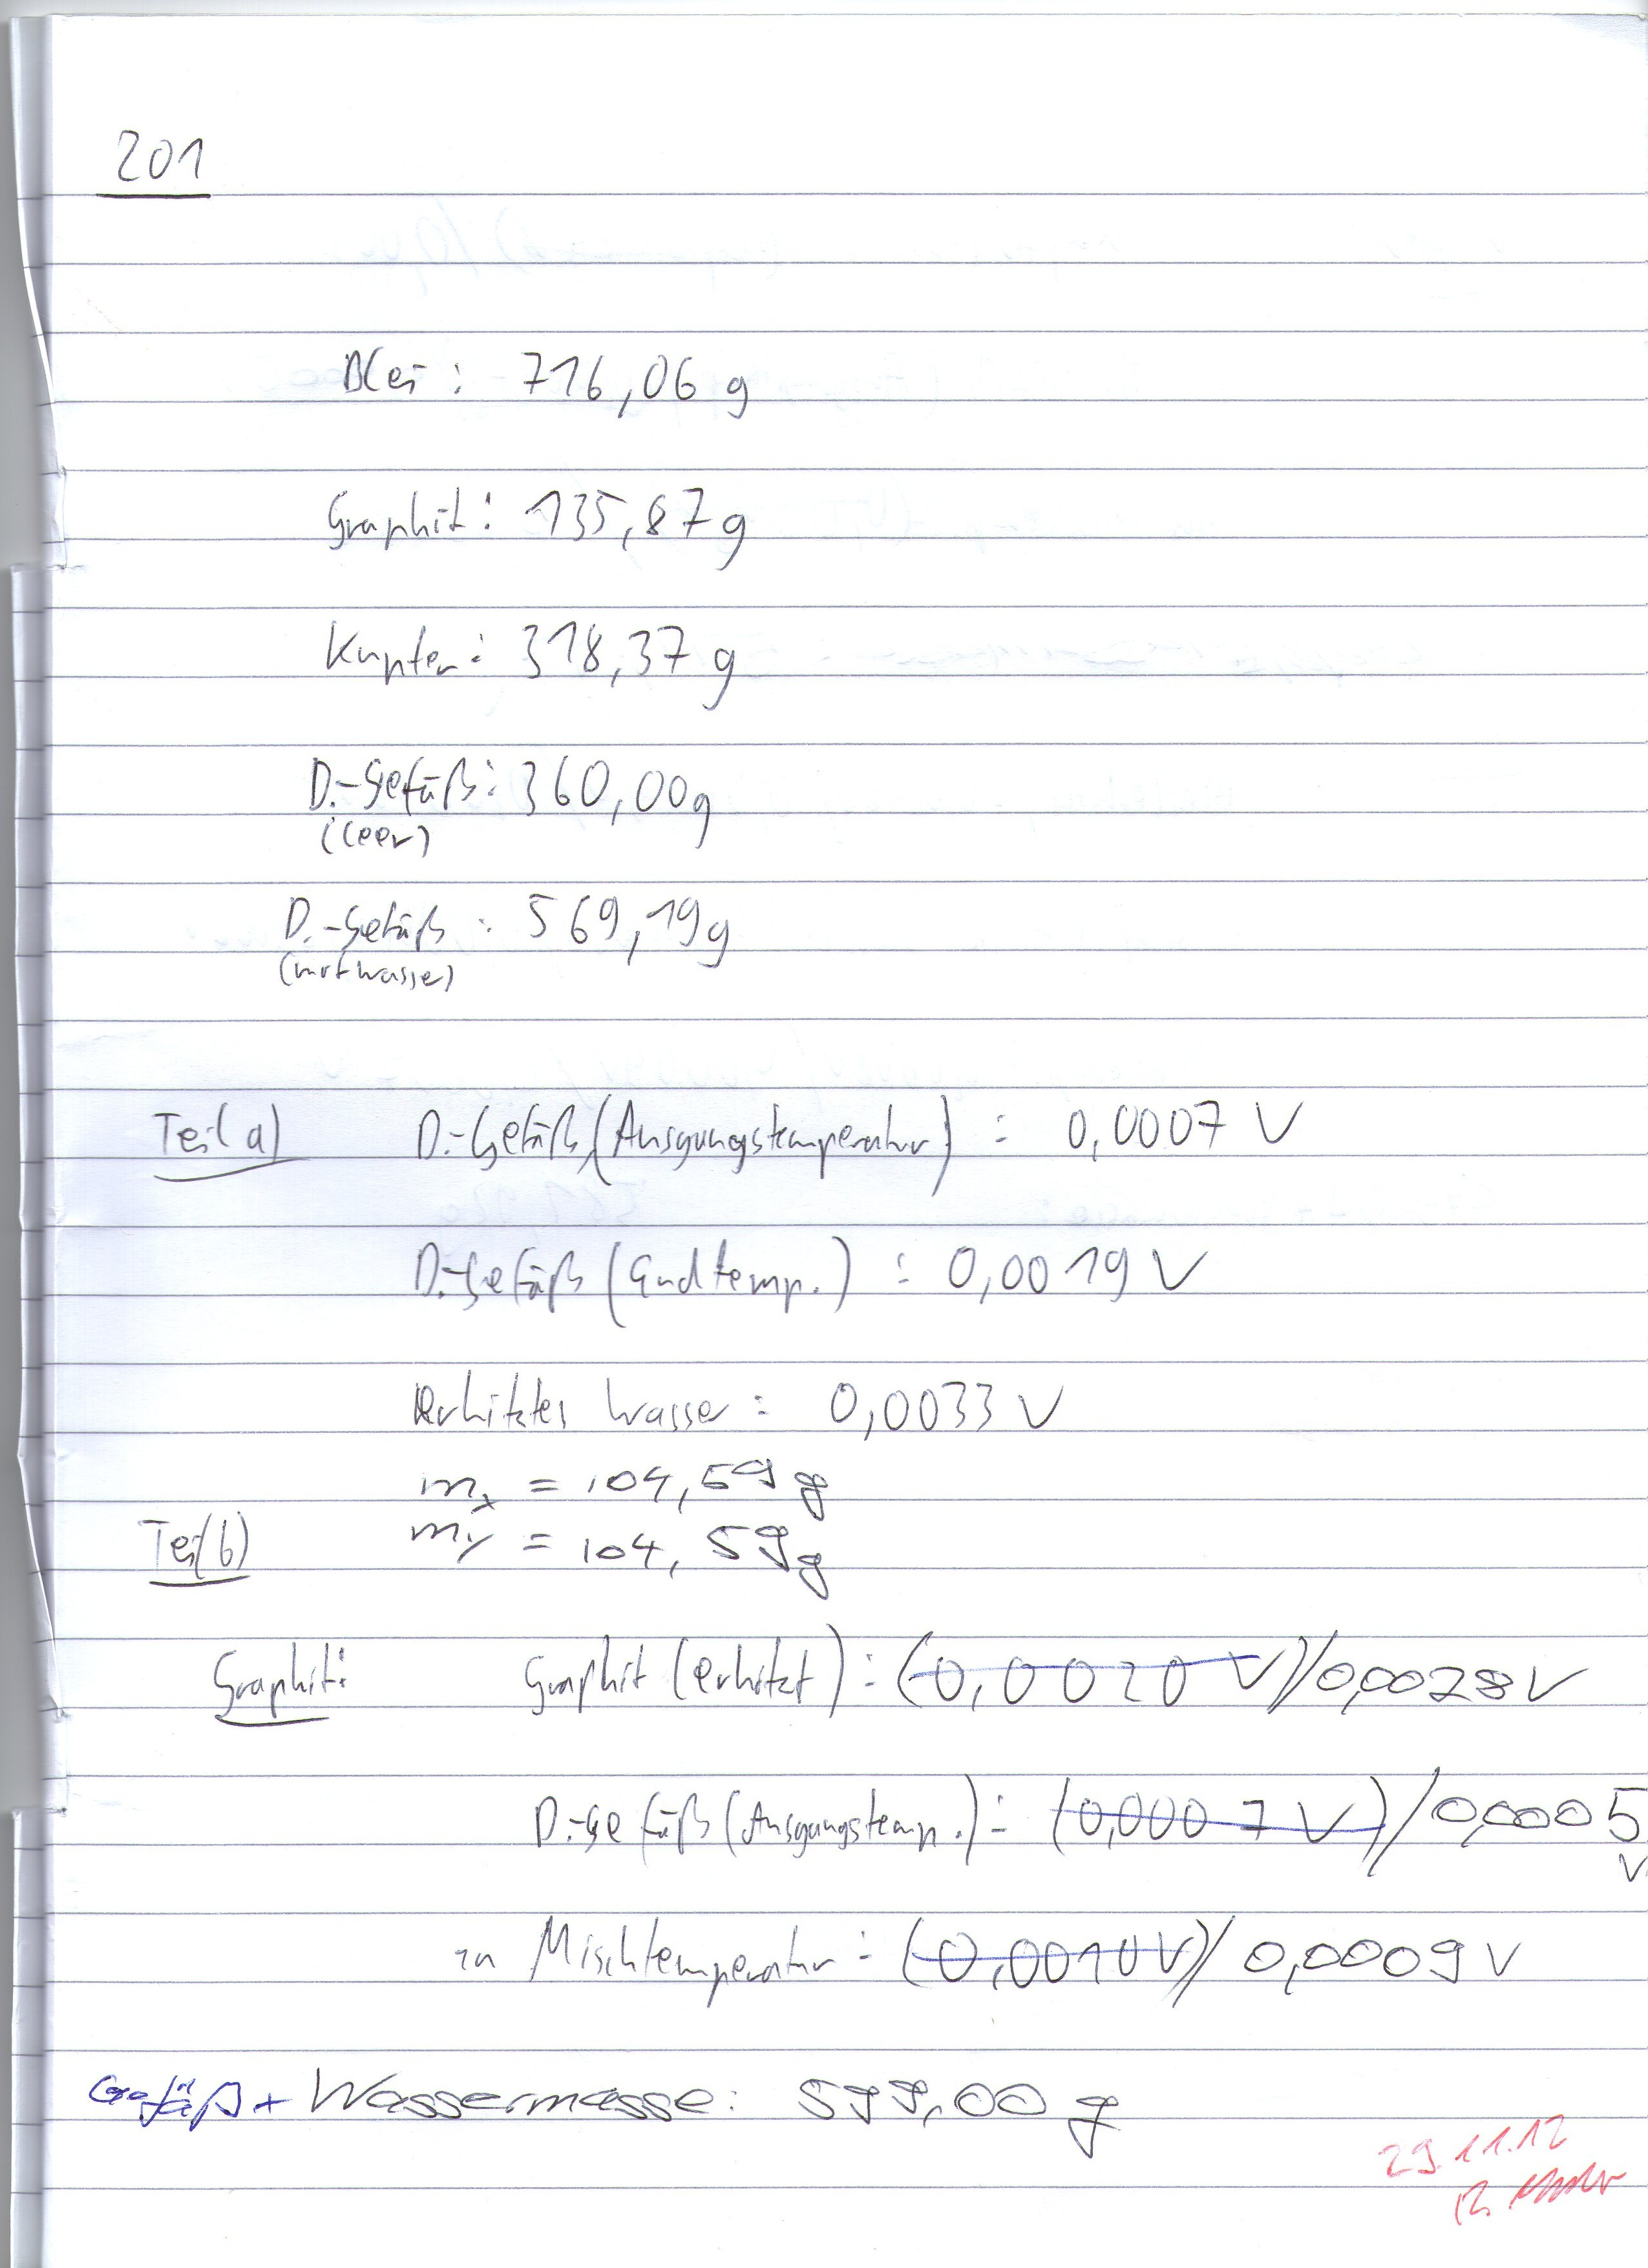
\includegraphics[scale=0.75]{img011.jpg}
\end{document}